% !TEX encoding = IsoLatin

% Prima riga per gli editor TeXShop, TeXWorks e TeXstudio per configurare codifica  ISO 8859-1
% La codifica di questo file deve essere ISO 8859-1 se si sceglie \usepackage[latin1]{inputenc}

\documentclass[
,cucitura
%,twoside
,corpo=13pt
]{toptesi}

%\usepackage[a-1b]{pdfx}
\usepackage{hyperref}
\hypersetup{%
    pdfpagemode={UseOutlines},
    bookmarksopen,
    pdfstartview={FitH},
    colorlinks,
    linkcolor={blue},
    citecolor={red},
    urlcolor={blue}
  }
% \documentclass[11pt,twoside,oldstyle,autoretitolo,classica,greek]{toptesi}   % \usepackage[or]{teubner}
% Nel seguito laurea "quinquennale" sta anche per "specialistica" o "magistrale

\usepackage[latin1]{inputenc}
\usepackage{titlesec}
\usepackage{lipsum} % I don't know what is this ;)
\input{commands.tex}
\usepackage{dirtytalk}
\usepackage{amsmath}
\usepackage{fancyvrb}
\usepackage{graphicx} 
\usepackage{pdfoverlay,textpos} % this for  the images



\usepackage{listings} %for code snippets
\usepackage{xcolor}   % for code snippets

%New colors defined below
\definecolor{codegreen}{rgb}{0,0.6,0}
\definecolor{codegray}{rgb}{0.5,0.5,0.5}
\definecolor{codepurple}{rgb}{0.58,0,0.82}
\definecolor{backcolour}{rgb}{0.95,0.95,0.92}

%Code listing style named "mystyle"
\lstdefinestyle{mystyle}{
  backgroundcolor=\color{backcolour}, commentstyle=\color{codegreen},
  keywordstyle=\color{magenta},
  numberstyle=\tiny\color{codegray},
  stringstyle=\color{codepurple},
  basicstyle=\ttfamily\footnotesize,
  breakatwhitespace=false,         
  breaklines=true,                 
  captionpos=b,                    
  keepspaces=true,                 
  numbers=left,                    
  numbersep=5pt,                  
  showspaces=false,                
  showstringspaces=false,
  showtabs=false,                  
  tabsize=2
}
\lstset{style=mystyle}

\usepackage{tikz}
\usetikzlibrary{positioning}
\usepackage{tcolorbox}
\usetikzlibrary{shapes.geometric, arrows, snakes, backgrounds, automata}
\tikzstyle{startstop} = [rectangle, rounded corners, minimum width=3cm, minimum height=1cm,text centered, draw=black, fill=red!30]
\tikzstyle{io} = [trapezium, trapezium left angle=70, trapezium right angle=110, minimum width=1cm, minimum height=1cm, text centered, draw=black, fill=blue!30]
\tikzstyle{process} = [rectangle, minimum width=1cm, minimum height=1cm, text centered, draw=black, fill=orange!30]
\tikzstyle{decision} = [diamond, minimum width=1cm, minimum height=1cm, text centered, draw=black, fill=green!30]
\tikzstyle{arrow} = [thick,->,>=stealth]
%\tikzstyle{state} = [fill=blue!30]
\tikzstyle{state}=[circle,draw=blue!50,fill=blue!20,thick]
\tikzstyle{transition}=[rectangle,draw=black!50,fill=black!20,thick]


\usepackage{blindtext}
%Image-related packages
\usepackage{graphicx}
\usepackage{subcaption}
\usepackage[export]{adjustbox}
\usepackage{wrapfig}
%------------------------------
%Table-related commands
\usepackage{array}
\usepackage[table]{xcolor}
\setlength{\arrayrulewidth}{1mm}
\setlength{\tabcolsep}{18pt}
\renewcommand{\arraystretch}{1.5}
\newcolumntype{s}{>{\columncolor[HTML]{AAACED}} p{3cm}}
%-------------------------------------------------------



\usepackage[acronym]{glossaries}
\makeglossaries
\newacronym{neural-network}{NN}{Neural Network}
\newacronym{machine-learning}{ML}{Machine Learning}
\newacronym{named-entity-recognition}{NER}{Named Entity Recognition}
\newacronym{natural-language-processing}{NLP}{Natural Language Processing}
\newacronym{human-in-the-loop}{HITL}{Human In The Loop}
\newacronym{True Positive}{TP}{True Positive}
\newacronym{False Positive}{FP}{False Positive}
\newacronym{True Negative}{TN}{True Negative}
\newacronym{False Negative}{FN}{False Negative}
\newacronym{Precision}{P}{Precision}
\newacronym{Recall}{R}{Recall}
\newacronym{F1-score}{F1}{F1-score}
\newacronym{Accuracy}{A}{Accuracy}
\newacronym{Pubblica Amministrazione}{PA}{Pubblica Amministrazione}
\newacronym{Codice Identificativo di Gara}{CIG}{Codice Identificativo di Gara}
\newacronym{Codice Unico di Progetto}{CUP}{Codice Unico di Progetto}
\newacronym{societa-soa}{SOA}{Societ� Organismi di Attestazione}
  \newacronym{OG-1}{OG-1}{Edifici civili e industriali}
  \newacronym{OG-2}{OG-2}{Restauro e manutenzione dei beni immobili sottoposti a tutela}
\newacronym{OG-3}{OG-3}{Strade, autostrade, ponti, viadotti, ferrovie, metropolitane}
\newacronym{OG-4}{OG-4}{Opere d'arte nel sottosuolo}
\newacronym{OG-5}{OG-5}{Dighe}
\newacronym{OG-6}{OG-6}{Acquedotti, gasdotti, oleodotti, opere di irrigazione e di evacuazione}
\newacronym{OG-7}{OG-7}{Opere marittime e lavori di dragaggio}
\newacronym{OG-8}{OG-8}{Opere fluviali, di difesa, di sistemazione idraulica e di bonifica}
\newacronym{OG-9}{OG-9}{Impianti per la produzione di energia elettrica}
\newacronym{OG-10}{OG-10}{Impianti per la trasformazione alta/media tensione e per la distribuzione di energia elettrica in corrente alternata e continua ed impianti di pubblica illuminazione}
  \newacronym{OG-11}{OG-11}{Impianti tecnologici}
  \newacronym{OG-12}{OG-12}{Opere ed impianti di bonifica e protezione ambientale}
  \newacronym{OG-13}{OG-13}{Opere di ingegneria naturalistica}
  \newacronym{OS-1}{OS-1}{Lavori in terra}
  \newacronym{OS-2-A}{OS-2-A}{Superfici decorate di beni immobili del patrimonio culturale e beni culturali mobili di interesse storico, artistico, archeologico ed etnoantropologico}
  \newacronym{OS-2-B}{OS-2-B}{Beni culturali mobili di interesse archivistico e librario}
  \newacronym{OS-3}{OS-3}{Impianti idrico-sanitario, cucine, lavanderie}
  \newacronym{OS-4}{OS-4}{Impianti elettromeccanici trasportatori}
  \newacronym{OS-5}{OS-5}{Impianti pneumatici e antintrusione}
  \newacronym{OS-6}{OS-6}{Finiture di opere generali in materiali lignei, plastici, metallici e vetrosi}
  \newacronym{OS-7}{OS-7}{Finiture di opere generali di natura edile e tecnica}
  \newacronym{OS-8}{OS-8}{Opere di impermeabilizzazione}
  \newacronym{OS-9}{OS-9}{Impianti per la segnaletica luminosa e la sicurezza del traffico}
  \newacronym{OS-10}{OS-10}{Segnaletica stradale non luminosa}
  \newacronym{OS-11}{OS-11}{Apparecchiature strutturali speciali}
  \newacronym{OS-12-A}{OS-12-A}{Barriere stradali di sicurezza}
  \newacronym{OS-12-B}{OS-12-B}{Barriere paramassi, fermaneve e simili}
  \newacronym{OS-13}{OS-13}{Strutture prefabbricate in cemento armato}
  \newacronym{OS-14}{OS-14}{Impianti di smaltimento e recupero rifiuti}
  \newacronym{OS-15}{OS-15}{Pulizia di acque marine, lacustri, fluviali}
  \newacronym{OS-16}{OS-16}{Impianti per centrali produzione energia elettrica}
  \newacronym{OS-17}{OS-17}{Linee telefoniche ed impianti di telefonia}
  \newacronym{OS-18-A}{OS-18-A}{Componenti strutturali in acciaio}
  \newacronym{OS-18-B}{OS-18-B}{Componenti per facciate continue}
  \newacronym{OS-19}{OS-19}{Impianti di reti di telecomunicazione e di trasmissioni e trattamento}
  \newacronym{OS-20-A}{OS-20-A}{Rilevamenti topografici}
  \newacronym{OS-20-B}{OS-20-B}{Indagini geognostiche}
  \newacronym{OS-21}{OS-21}{Opere strutturali speciali}
  \newacronym{OS-22}{OS-22}{Impianti di potabilizzazione e depurazione}
  \newacronym{OS-23}{OS-23}{Demolizione di opere}
  \newacronym{OS-24}{OS-24}{Verde e arredo urbano}
  \newacronym{OS-25}{OS-25}{Scavi archeologici}
  \newacronym{OS-26}{OS-26}{Pavimentazioni e sovrastrutture speciali}
  \newacronym{OS-27}{OS-27}{Impianti per la trazione elettrica}
  \newacronym{OS-28}{OS-28}{Impianti termici e di condizionamento}
  \newacronym{OS-29}{OS-29}{Armamento ferroviario}
  \newacronym{OS-30}{OS-30}{Impianti interni elettrici, telefonici, radiotelefonici e televisivi}
  \newacronym{OS-31}{OS-31}{Impianti per la mobilità sospesa}
  \newacronym{OS-32}{OS-32}{Strutture in legno}
  \newacronym{OS-33}{OS-33}{Coperture speciali}
  \newacronym{OS-34}{OS-34}{Sistemi antirumore per infrastrutture di mobilità}
  \newacronym{OS-35}{OS-35}{Interventi a basso impatto ambientale}
  \newacronym{I}{I classifica}{fino a euro 258.000}
  \newacronym{II}{II classifica}{fino a euro 516.000}
  \newacronym{III}{III classifica}{fino a euro 1.033.000}
  \newacronym{III-bis}{III bis classifica}{fino a euro 1.500.000}
  \newacronym{IV}{IV classifica}{fino a euro 2.582.000}
  \newacronym{IV-bis}{IV bis classifica}{fino a euro 3.500.000}
  \newacronym{V}{V classifica}{fino a euro 5.165.000}
  \newacronym{VI}{VI classifica}{fino a euro 10.329.000}
  \newacronym{VII}{VII classifica}{fino a euro 15.494.000}
  \newacronym{VIII}{VIII classifica}{oltre euro 15.494.000}







%\usepackage[a-1b]{pdfx}
%\hypersetup{%
%    pdfpagemode={UseOutlines},
%    bookmarksopen,
%    pdfstartview={FitH},
%    colorlinks,
%    linkcolor={blue},
%    citecolor={green},
%    urlcolor={blue}
%  }
%
% per numerare e far comparire nell'indice anche le sezioni di quarto livello
% SCONSIGLIATO! da usarsi solo in caso di estrema necessit�
%\setcounter{secnumdepth}{4}% section-numbering-depth
%\setcounter{tocdepth}{4}% TOC-numbering-depth (TOC=Table-Of-Content)

%\setbindingcorrection{3mm}


%******FUNZIONALIT� STANDARD DI TOPTESI UTILIZZABILI DOPO BEGIN DOCUMENT*********************************************

%%% scegliere la propria facolt� (solo PRIMA dell'AA 2012-2013) \facolta[III]{Ingegneria dell'Informazione} \facolta[IV]{Organizzazione d'Impresa\\e Ingegneria Gestionale}

%\monografia{Estrazione di dati della P.A.}% per la laurea triennale
%\titolo{Estrazione di dati della P.A.}% per la laurea quinquennale e il dottorato
%%\sottotitolo{Metodo dei satelliti medicei}

%%% scegliere il proprio corso
%
%\corsodilaurea{Ingegneria dell'Organizzazione d'Impresa}% per la laurea di primo e secondo livello
%\corsodilaurea{Ingegneria Logistica e della Produzione}% per la laurea di primo e secondo livello
%\corsodilaurea{Ingegneria Gestionale}% per la laurea di primo e secondo livello
%\corsodilaurea{Ingegneria Informatica}% per la laurea di primo e secondo livello
%\corsodidottorato{Meccanica}% per il dottorato

%\candidato{Davide \textsc{Maietta}}% per tutti i percorsi
%\secondocandidato{Evangelista \textsc{Torricelli}}% per la laurea magistrale solamente
%\direttore{prof. Albert Einstein}% per il dottorato
%\coordinatore{prof. Albert Einstein}% per il dottorato
%\relatore{prof.\ Maurizio Morisio}% per la laurea e il dottorato
%\secondorelatore{dipl.~ing.~Werner von Braun}% per la laurea magistrale
%\terzorelatore{{\tabular{@{}l}dott.\ Neil Armstrong\\prof. Maria Rossi\endtabular}}% per la laurea magistrale
%\tutore{ing.~Karl Von Braun}% per il dottorato
%\tutoreaziendale{dott.\ ing.\ Giovanni Giacosa} % solo per la laurea di secondo livello con tesi svolta in azienda
%\NomeTutoreAziendale{Supervisore aziendale\\Centro Ricerche FIAT}
%\sedutadilaurea{Agosto 1615}% per la laurea quinquennale
%\esamedidottorato{Novembre 1610}% per il dottorato
%\sedutadilaurea{\textsc{Novembre} 2017}% per la laurea triennale
%\sedutadilaurea{\textsc{Anno~accademico} 1615-1616}% per la laurea magistrale
%\annoaccademico{1615-1616}% solo con l'opzione classica
%\annoaccademico{2006-2007}% idem
%\ciclodidottorato{XV}% per il dottorato
%\logosede{logopolito}
%
%\AdvisorName{Supervisors}
%\newtheorem{osservazione}{Osservazione}% Standard LaTeX
%\errorcontextlines=9
%\frontespizio
%\paginavuota
%\newpage
%\advance\voffset -5mm
%\advance\textheight 30mm
%\begin{dedica}
%\end{dedica}
%\dagger
%\sommario
%Inserire qui un breve sommario della tesi.
%\ringraziamenti
%Opzionali, solo nel caso si sia ricevuto un aiuto speciale e particolarmente rilevante.
%% inserire sempre nella tesi per la laurea di I livello, perch� il nome dei tutori non � indicato sul frontespizio.
%Il lavoro descritto in questa monografia � stato svolto sotto la supervisione
%del Prof. (tutore accademico)% inserire sempre il nome del tutore accademico
% e dell'Ing. (tutore aziendale)% inserire solo se la monografia � relativa ad un tirocinio.

%\tablespagetrue 
%\figurespagetrue 

\begin{document}
\ateneo{Politecnico di Torino}
\titolo{Estrazione di entit� da testi della Pubblica Amministrazione}% per la laurea quinquennale e il dottorato
\logosede{logopolito}
\corsodilaurea{Ingegneria Informatica}% per la laurea di primo e secondo livello
\candidato{Davide \textsc{Maietta}}% per tutti i percorsi
\relatore{prof. Maurizio Morisio}
%\secondorelatore{dipl.~ing.~Werner von Braun}
    \terzorelatore{\tabular{@{}l}
	\textbf{Correlatore:}\\
    dott. Giuseppe Rizzo\\[0.5ex]
	\textbf{Correlatore:}\\
    dott. Davide Allavena\\
%	\textbf{Correlatore:}\\
%    dott.~Mario Rossi\\[0.5ex]
%	\textbf{Correlatore:}\\
%    dott.~Piero Neri
    \endtabular}
\sedutadilaurea{\textsc{Dicembre} 2021}% per la laurea triennale
\errorcontextlines=9
\frontespizio
\paginavuota
\newpage
\advance\voffset -5mm
\advance\textheight 30mm
%\begin{dedica}
%\end{dedica}
%\sommario
%SAR� BREVE
\indici
\mainmatter

%\titleformat{\chapter}[display]  {\normalfont\bfseries}{}{0pt}{\Large} %evita la dicitura "capitolo" fornendo solo la numerazione

% !TEX encoding = IsoLatin 

% Affinch� gli accenti vengano accettati, assicurati che la codifica di questo file
% sia ISO 8859-1

% PER OTTENERE IL PDF, digitare da terminale
% ./makepdfplease
% 

\chapter{Introduzione}
L'avanzamento tecnologico delle telecomunicazioni negli ultimi decenni ha permesso alle persone di recuperare dati e informazioni provenienti dai luoghi pi� disparati e ad una velocit� di approvvigionamento praticamente nulla: se prima di Internet l'unico modo di ricevere un documento ufficiale era farne richiesta all'ufficio competente, ora le documentazioni possono essere normalmente a disposizione in rete. Gli utenti della rete hanno a disposizione una mole cos� grande di documenti e informazioni che gli � praticamente impossibile visionare la totalit� di questi dati.
In questo contesto l'esigenza di estrarre dati da documenti � sempre pi� sentita, soprattutto quando si voglia fare una cernita dei documenti contenenti specifiche informazioni di proprio interesse.
Questa tesi ha come scopo effettuare un'estrazione di dati da un insieme di documenti della \acrfull{Pubblica Amministrazione}; pi� precisamente i documenti appartengono al contesto dei bandi pubblici e i dati da cercare sono tutte quelle informazioni che impongono dei requisiti ai possibili partecipanti di gara. 
Il lavoro � strutturato come segue: al capitolo secondo si descrivono i bandi pubblici e dati SOA in essi contenuti; 
al capitolo terzo si presenta il problema della ricerca di tali dati formalizzata come un problema di Named Entity Extraction.
Al capitolo quarto viene svolta una rassegna di lavori correlati, che vertono sulle metodologie di estrazione di dati; 
dopodich� tali metodologie vengono implementate al capitolo quinto. 
In questo contesto si provano approcci tecnologici diversi, nella fattispecie l'uso delle regular expressions e delle reti neurali. Di entrambe le tecnologie vengono delineati punti di forza e di debolezza, per poi investigare se sia preferibile l'una delle due o se invece sia possibile un compromesso che valorizzi il meglio di entrambe.
Al capitolo sesto si introduce un approccio ibrido configurato come Human In The Loop, che viene proposto come 
soluzione vantaggiosa rispetto alle tecnologie singole considerate inizialmente. Nell'ultimo capitolo sono esposte le conclusioni e le possibilit� di sviluppi successivi per questo lavoro di ricerca.
% !TEX encoding = IsoLatin 

% Affinch� gli accenti vengano accettati, assicurati che la codifica di questo file
% sia ISO 8859-1

% PER OTTENERE IL PDF, digitare da terminale
% ./makepdfplease
% 

% !TEX encoding = IsoLatin 

% Affinch� gli accenti vengano accettati, assicurati che la codifica di questo file
% sia ISO 8859-1

% PER OTTENERE IL PDF, digitare da terminale
% ./makepdfplease
% 
% !TEX encoding = IsoLatin 

% Affinch� gli accenti vengano accettati, assicurati che la codifica di questo file
% sia ISO 8859-1

% PER OTTENERE IL PDF, digitare da terminale
% ./makepdfplease
% 



\chapter{Estrazione di dati da testi della pubblica amministrazione}
%\chapter[Estrazione di dati da testi della pubblica amministrazione][]{1. Estrazione di dati da testi della pubblica amministrazione}
%IoT \cite{friis} basically refers to ....\\
%\ac{IoT} basically refers to ....\\

%\section{Introduzione}
L'avanzamento tecnologico delle telecomunicazioni negli ultimi decenni ha permesso alle persone di recuperare dati e informazioni provenienti dai luoghi pi� disparati e ad una velocit� di approvvigionamento praticamente nulla: se prima di Internet l'unico modo di ricevere un documento ufficiale era farne richiesta all'ufficio competente, ora le documentazioni possono essere normalmente a disposizione in rete. Gli utenti della rete hanno a disposizione una mole cos� grande di documenti e informazioni che gli � praticamente impossibile visionare la totalit� di questi dati.
In questo contesto l'esigenza di estrarre dati da documenti � sempre pi� sentita, soprattutto quando si voglia fare una cernita dei documenti contenenti specifiche informazioni di proprio interesse.
Questa tesi ha come scopo effettuare un'estrazione di dati da un insieme di documenti della \acrfull{Pubblica Amministrazione}; pi� precisamente i documenti appartengono al contesto dei bandi pubblici e i dati da cercare sono tutte quelle informazioni che impongono dei requisiti ai possibili partecipanti di gara. 
In questo contesto si provano approcci tecnologici diversi, nella fattispecie l'uso delle regular expressions e delle reti neurali; di entrambe le tecnologie si delineano punti di forza e svantaggi, per poi investigare se sia preferibile l'una delle due o se invece sia possibile un compromesso che valorizzi il meglio di entrambe. 
Nella sezione che segue delineeremo in dettaglio 

%\section{Contesto}

\section{Gare d'appalto}
Tra le funzioni di uno Stato vi sono la costruzione, la manutenzione e la messa in sicurezza delle infrastrutture di pubblica utilit�, quali ad esempio gli edifici pubblici, le reti di telecomunicazione, le strade e gli ospedali di cui beneficiano i cittadini.
La \acrlong{Pubblica Amministrazione}, dovendo garantire una quantit� cos� grande di infrastrutture, non esegue i lavori direttamente, ma ne delega l'attuazione pratica a delle imprese private con un appalto pubblico.
L'appalto � un contratto con il quale una parte, detta parte appaltatrice, assume, \say{con organizzazione dei mezzi necessari e con gestione a proprio rischio, l'obbligazione di compiere in favore di un'altra (committente o appaltante) un'opera o un servizio}\cite{basacchi2013codice}.
Gli appalti pubblici sono dunque un modo per eseguire delle opere pubbliche pagando delle imprese private per la realizzazione vera e propria; la \acrshort{Pubblica Amministrazione} deve per� assicurarsi che:
l'impresa abbia le conoscenze per portare a termine l'opera rispettando degli standard tecnici, ossia seguendo la \textbf{regola d'arte};
l'impresa gestisca i lavori in maniera competitiva, senza comportare sprechi ingiustificati di soldi pubblici;
l'impresa riesca a reggere lo sforzo finanziario che l'opera comporta, sia per quanto riguarda l'approvvigionamento dei materiali, sia per quanto riguarda il costo del lavoro.
L'assegnazione di un progetto si avvale di apposita gara d'appalto, che ha come obbiettivo la selezione dell'impresa che meglio possa soddisfare questi requisiti di competenze tecniche, finanziarie e di competitivit� sul mercato.

\section{Identificativi di progetto e di gara}
Nell'ambito di una gara d'appalto, il progetto pu� essere composto da pi� parti singole chiamate lotti; l'assegnazione di un lotto � indipendente dagli altri, per cui diversi lotti di un progetto possono essere assegnati ad aziende differenti nell'ambito della stessa gara d'appalto.
I documenti che andiamo ad analizzare riportano una serie di informazioni di nostro interesse, quali:
\begin{itemize}
\item il \textbf{\acrfull{Codice Unico di Progetto}}, che descrive univocamente il progetto d'investimento pubblico;  � un identificativo alfanumerico di quindici caratteri;
\item il \textbf{\acrfull{Codice Identificativo di Gara}}, che indica in maniera univoca il lotto;
 � un identificativo alfanumerico di dieci caratteri;
\end{itemize}

\section{Lavori e importi}
La gara d'appalto deve indicare in maniera evidente e inoppugnabile quali competenze tecniche e quali capacit� finanziarie sono ritenute requisiti fondamentali per la partecipazione; qualsiasi ambiguit� nei requisiti di una gara potrebbe dare adito a ricorsi e quindi a rallentare la gara stessa. 
Il bisogno di requisiti oggettivi ha motivato l'introduzione di apposite certificazioni fornite dalle 
\acrfull{societa-soa}, che prendono il nome di \say{certificati SOA} o \say{attestazioni SOA}.
Tali attestazioni si dividono in due macrogruppi:
\begin{itemize}
\item \textbf{Categorie di lavori:} individuano le categorie di opere dal punto di vista tecnico;
\item \textbf{Classifiche di importi:} individuano i livelli di capacit� finanziaria.
\end{itemize}
Un bando di gara esprimer� i requisiti di progetto sotto forma di categorie e classifiche SOA, per cui un'azienda che voglia  essere ammessa alla gara dovr� possedere le attestazioni SOA richieste.









\section{Tassonomia SOA}
Le Categorie sono suddivise in due macro-categorie: opere generali e opere specializzate,  rispettivamente identificate dagli acronimi \say{OG} e \say{OS}; sono individuate 13 categorie di Opere Generali e 39 categorie di Opere Specializzate.
Le Classifiche d'importo, in numero di dieci, sono rese come numeri ordinali romani. 


\subsection{Categorie di opere generali}
\begin{itemize}
  \item \acrshort{OG-1}, \acrlong{OG-1}
  \item \acrshort{OG-2}, \acrlong{OG-2}
\item \acrshort{OG-3}, \acrlong{OG-3}
\item \acrshort{OG-4}, \acrlong{OG-4}
\item \acrshort{OG-5}, \acrlong{OG-5}
\item \acrshort{OG-6}, \acrlong{OG-6}
\item \acrshort{OG-7}, \acrlong{OG-7}
\item \acrshort{OG-8}, \acrlong{OG-8}
\item \acrshort{OG-9}, \acrlong{OG-9}
\item \acrshort{OG-10}, \acrlong{OG-10}
  \item \acrshort{OG-11}, \acrlong{OG-11}
  \item \acrshort{OG-12}, \acrlong{OG-12}
  \item \acrshort{OG-13}, \acrlong{OG-13}
\end{itemize}

\subsection{Categorie di opere specializzate}
\begin{itemize}
  \item \acrshort{OS-1}, \acrlong{OS-1}
  \item \acrshort{OS-2-A}, \acrlong{OS-2-A}
  \item \acrshort{OS-2-B}, \acrlong{OS-2-B}
  \item \acrshort{OS-3}, \acrlong{OS-3}
  \item \acrshort{OS-4}, \acrlong{OS-4}
  \item \acrshort{OS-5}, \acrlong{OS-5}
  \item \acrshort{OS-6}, \acrlong{OS-6}
  \item \acrshort{OS-7}, \acrlong{OS-7}
  \item \acrshort{OS-8}, \acrlong{OS-8}
  \item \acrshort{OS-9}, \acrlong{OS-9}
  \item \acrshort{OS-10}, \acrlong{OS-10}
  \item \acrshort{OS-11}, \acrlong{OS-11}
  \item \acrshort{OS-12-A}, \acrlong{OS-12-A}
  \item \acrshort{OS-12-B}, \acrlong{OS-12-B}
  \item \acrshort{OS-13}, \acrlong{OS-13}
  \item \acrshort{OS-14}, \acrlong{OS-14}
  \item \acrshort{OS-15}, \acrlong{OS-15}
  \item \acrshort{OS-16}, \acrlong{OS-16}
  \item \acrshort{OS-17}, \acrlong{OS-17}
  \item \acrshort{OS-18-A}, \acrlong{OS-18-A}
  \item \acrshort{OS-18-B}, \acrlong{OS-18-B}
  \item \acrshort{OS-19}, \acrlong{OS-19}
  \item \acrshort{OS-20-A}, \acrlong{OS-20-A}
  \item \acrshort{OS-20-B}, \acrlong{OS-20-B}
  \item \item \acrshort{OS-21}, \acrlong{OS-21}
  \item \acrshort{OS-22}, \acrlong{OS-22}
  \item \acrshort{OS-23}, \acrlong{OS-23}
  \item \acrshort{OS-24}, \acrlong{OS-24}
  \item \acrshort{OS-25}, \acrlong{OS-25}
  \item \acrshort{OS-26}, \acrlong{OS-26}
  \item \acrshort{OS-27}, \acrlong{OS-27}
  \item \acrshort{OS-28}, \acrlong{OS-28}
  \item \acrshort{OS-29}, \acrlong{OS-29}
  \item \acrshort{OS-30}, \acrlong{OS-30}
  \item \acrshort{OS-31}, \acrlong{OS-31}
  \item \acrshort{OS-32}, \acrlong{OS-32}
  \item \acrshort{OS-33}, \acrlong{OS-33}
  \item \acrshort{OS-34}, \acrlong{OS-34}
  \item \acrshort{OS-35}, \acrlong{OS-35}
\end{itemize}

\subsection{Classifiche importo }
\begin{itemize}
  \item \acrshort{I}, \acrlong{I}
  \item \acrshort{II}, \acrlong{II}
  \item \acrshort{III}, \acrlong{III}
  \item \acrshort{III-bis}, \acrlong{III-bis}
  \item \acrshort{IV}, \acrlong{IV}
  \item \acrshort{IV-bis}, \acrlong{IV-bis}
  \item \acrshort{V}, \acrlong{V}
  \item \acrshort{VI}, \acrlong{VI}
  \item \acrshort{VII}, \acrlong{VII}
  \item \acrshort{VIII}, \acrlong{VIII}
\end{itemize}  


% !TEX encoding = IsoLatin 

% Affinch� gli accenti vengano accettati, assicurati che la codifica di questo file
% sia ISO 8859-1

% PER OTTENERE IL PDF, digitare da terminale
% ./makepdfplease
% 





%\section{Casi d'uso delle attestazioni SOA}
Finora sono state descritte le attestazioni SOA ed � stato chiarito il ruolo fondamentale che queste certificazioni ricoprono negli appalti.
D'ora in avanti si intende descrivere l'uso di queste attestazioni da parte dei vari attori del mondo degli appalti:
\begin{enumerate}
  \item la \textbf{Pubblica Amministrazione}: produce il bando di gara, relativo ad un progetto identificato univocamente dal codice CUP ed eventualmente diviso in lotti, ognuno identificato da un codice CIG; nel bando di gara aggiunge i requisiti di Categorie SOA e le Classifiche economiche SOA, imponendo eventualmente vincoli temporali su tali certificati (\say{L'azienda deve risultare in possesso di tale certificato dal 2020}); il bando viene scritto in formato pdf e pubblicato sul sito dell'ente pubblico ( Comune, Provincia, Regione, Ministero, et cetera), che risulta in questo contesto essere l'appaltante;
\item l'\textbf{imprenditore}, o qualsivoglia candidato appaltatore: naviga i siti web della Pubblica Amministrazione alla ricerca di bandi di gara; per ogni bando di gara trovato, deve comprendere i requisiti SOA e accertarsi di poterli soddisfare; solo se dotato di idonea attestazione, potr� candidarsi ad essere appaltatore prendendo parte alla gara d'appalto.
\end{enumerate}
Sia chiaro che la P.A. pubblica anche altre tipologie di documenti, per cui � utile precisare che ci riferiamo a quell'insieme di documenti che descrivono gare e verbali d'appalto:  possiamo riferirci a questo insieme chiamandolo dominio d'appalto.
In questi due casi d'uso possiamo evidenziare una prima problematica: ogni ente pubblico ha un proprio sito web e la raccolta di documenti di appalti pu� essere un'attivit� lunga e dispersiva. Questo problema potrebbe essere risolto da un software di tipo web-crawler che navighi i siti web della pubblica amministrazione e raccolga tutti i documenti del dominio d'appalto in un dataset.
Esiste una seconda problematica da porre: ammesso che abbia a disposizione tutto il dataset del dominio degli appalti, l'imprenditore che � alla ricerca di un bando adatto alla sua specifica certificazione si trover� costretto a verificare per ogni documento se tale certificazione sia sufficiente per essere ammesso al bando; detto in altre parole, dovr� leggere e annotare manualmente tutti i documenti in base alle attestazioni SOA per poi scegliere il bando con l'annotazione SOA desiderata.
Questa problematica � decisamente noiosa, sia perch� la lettura toglie alla persona un ingente tempo di lavoro, sia perch� un compito del genere � perfettamente automatizzabile; d'ora in poi ci focalizzeremo su questa attivit� specifica.
L'idea di base � permettere alle imprese di migliorare la ricerca di possibili appalti rendendo questi documenti digitalmente navigabili in base alle attestazioni SOA: 
per l'imprenditore il caso d'uso 2 si ridurrebbe a cercare l'attestazione SOA desiderata per avere tutti e soli i bandi che la contemplino tra i requisiti.
La ricerca di attestazioni SOA in un testo � un problema di \textbf{Entity Extraction} (\textbf{EE}).
\paragraph{Formulazione del problema:}
\textit{
Dato un insieme di documenti in formato testuale appartenenti al dominio delle gare d'appalto, estrarre le attestazioni SOA ivi menzionate.
}

\section{Impostazione del problema}
%\subsection{Insiemi di valori}
L'impostazione del problema inizia con la definizione degli insiemi di valori possibili;
nel caso delle attestazioni SOA, seguendo la tassonomia esposta definiamo l'insieme delle Categorie e l'insieme delle Classifiche:
\begin{center}
Categorie = \{\say{OG-1} , \say{OG-2}, \say{OG-3}, \say{OG-4},
 \say{OG-5},\say{OG-6},\say{OG-7},\say{OG-8},
\end{center}
%\begin{center} \end{center} for each line to be displayed
\begin{center}
 \say{OG-9},\say{OG-10},\say{OG-11},\say{OG-12},
 \say{OG-13}, \say{OS-1},\say{OS-2A},\say{OS-2B},
 \say{OS-3},
\end{center}
\begin{center}
 \say{OS-4},\say{OS-5},\say{OS-6},
 \say{OS-7},\say{OS-8},\say{OS-9},\say{OS-10},
 \say{OS-11},\say{OS-12A},
\end{center}
\begin{center}
 \say{OS-12B}, \say{OS-13},
 \say{OS-14},\say{OS-15},\say{OS-16},\say{OS-17},
 \say{OS-18A},\say{OS-18B},
\end{center}
\begin{center}
 \say{OS-19},
 \say{OS-20A},
 \say{OS-20B},\say{OS-21},\say{OS-22},\say{OS-24},
 \say{OS-25}, \say{OS-26}, 
\end{center}
\begin{center}
 \say{OS-27}, \say{OS-28},
 \say{OS-29}, \say{OS-30}, \say{OS-31}, \say{OS-32},
 \say{OS-33}, \say{OS-34}, 
 \say{OS-35} \}
\end{center}
%\parbox{\textwidth}{
%Categorie = \{\say{OG-1} , \say{OG-2}, \say{OG-3}, \say{OG-4},
% \say{OG-5},\say{OG-6},\say{OG-7},\say{OG-8},\\
% \say{OG-9},\say{OG-10},\say{OG-11},\say{OG-12},
% \say{OG-13}, \say{OS-1},\say{OS-2A},\say{OS-2B},
% \say{OS-3},\\
% \say{OS-4},\say{OS-5},\say{OS-6},
% \say{OS-7},\say{OS-8},\say{OS-9},\say{OS-10},
% \say{OS-11},\say{OS-12A},\\
% \say{OS-12B}, \say{OS-13},
% \say{OS-14},\say{OS-15},\say{OS-16},\say{OS-17},
% \say{OS-18A},\say{OS-18B},\\
% \say{OS-19},
% \say{OS-20A},
% \say{OS-20B},\say{OS-21},\say{OS-22},\say{OS-24},
% \say{OS-25}, \say{OS-26}, \\
% \say{OS-27}, \say{OS-28},
% \say{OS-29}, \say{OS-30}, \say{OS-31}, \say{OS-32},
% \say{OS-33}, \say{OS-34}, 
% \say{OS-35} \}
% }
\begin{center}
Classifiche = \{\say{I}, \say{II}, \say{III}, \say{IV}, \say{IV-bis}, \say{V}, \say{VI}, \say{VII}, \say{VIII} \};
\end{center}

In definitiva, il sistema indicher� le informazioni estratte in base all'insieme Categorie e Classifiche cos� definiti. 
\subsection{Formato dei dati estratti}
Pi� in generale, per ogni attestazione SOA che il sistema individuer� in un documento, dovr� indicare varie informazioni:
\begin{itemize}
    \item la porzione di testo in cui l'attestazione SOA � individuata;
    \item la categoria riconosciuta;
    \item la classifica riconosciuta;
    \item lo score, ossia il grado di accuratezza dell'output.
\end{itemize}

\paragraph{soa\_extracted\_tuple} = [  (start\_offset\_cat, end\_offset\_cat), (categoria, classifica), score)
            ]

\section{Valutazione dei dati estratti}
Quando il sistema collega la stringa "o.g. 1" all'elemento OG-1, sta effettuando una classificazione: sta classificando un dato come appartenente alla classe delle istanze di OG-1.
Il sistema di estrazione dati effettua una classificazione su ogni porzione di testo individuata; ogni porzione di testo pu� essere collegata alla classe di uno dei valori SOA.
Tipicamente, in un problema di classificazione l'output pu� essere valutato come segue:
\begin{itemize}
    \item True Positive(TP), se l'elemento � stato assegnato correttamente alla classe;
    \item False Positive(FP), se l'elemento � stato assegnato erroneamente alla classe;
    \item True Negative(TN), se l'elemento non � stato assegnato alla classe perch� non vi andava assegnato;
    \item False Negative(FN), se l'elemento non � stato assegnato alla classe ma vi andava assegnato.
\end{itemize}

Ogni output del sistema verr� valutato in termini di TP-FP-TN-FN; questo permetter� di calcolare la bont� del sistema in termini di:

\paragraph{Precision} = (TP)/(TP + FP )
\paragraph{Recall} = (TP)/(TP + FN )
\paragraph{Accuracy} = (TP + TN)/(TP + TN + FP + FN)

\section{Ground truth}
Per ogni istanza di testo assegnato ad una classe, bisogna affermare se la classificazione data costituisce true positive, false positive, true negative o false negative; questo vuol dire che, per valutare la bont� di una classificazione, abbiamo bisogno di stabilire quale sia la classificazione giusta.
Il sistema che stiamo considerando effettua un'estrazione di dati, classificandoli come elementi delle attestazioni SOA; per valutare la bont� del sistema abbiamo dunque bisogno di stabilire per ogni porzione di testo l'output giusto, ovvero di definire la \textbf{verit�} in base alla quale valutare il sistema.
La \textbf{Ground Truth} � dunque l'output corretto che ci si aspetterebbe dal sistema; e come tale indicher�, per ogni porzione di documento, l'attestazione "giusta" che il sistema avrebbe dovuto estrarre.
Un sistema di apprendimento dotato di Ground Truth appartiene all'approccio detto \textbf{Apprendimento Supervisionato}. 
La ground truth verr� poi confrontata con l'output del sistema e permetter� di classificare ogni tupla dell'output come true positive, false positive, true negative, false negative.
Una volta contrassegnata ogni tupla dell'output come tp/fp/tn/fn, sar� possibile calcolare Precision, Recall e Accuracy.


\section{Tecniche di estrazione}
Di seguito si espongono due approcci principali per l'estrazione di dati:
\begin{itemize}
    \item l'uso di regular expression;
    \item l'uso di tecniche di machine learning.
\end{itemize}
Mostreremo che hanno differenti punti di forza, differenti punti di debolezza e confronteremo i risultati di entrambe le tecnologie.

% !TEX encoding = IsoLatin 

% Affinch� gli accenti vengano accettati, assicurati che la codifica di questo file
% sia ISO 8859-1

% PER OTTENERE IL PDF, digitare da terminale
% ./makepdfplease
% 




%\section{Impiego delle regular expression}
%\section{Difficolt� insite nelle regex}
Le espressioni regolari sono usatissime nel mondo della programmazione: 
si stima che siano utilizzate in \say{pi� di un terzo dei progetti Python e Javascript} \cite{RegexesAreHard}.
La loro grande diffusione non vuol dire per� che costituiscano una tecnologia sicura da utilizzare, poich� presentano
problematiche di leggibilit�, scarsit� di documentazione, difficile manutenibilit� e problemi di sicurezza non da poco conto.
\paragraph{Leggibilit�: } un grave problema delle regex � che, rappresentando dei pattern alfanumerici sintetizzati all'estremo, risultino incomprensibili alla lettura; gli sviluppatori non sono immuni a questo problema ed anche per 
loro risalire al pattern alfanumerico partendo da una regex pu� essere un compito scomodo.
\paragraph{Documentazione: } nel mondo della programmazione � consolidata la pratica di documentare i passaggi meno 
leggibili di un algoritmo; nel caso delle regular expression, queste sono inserite negli algoritmi sotto forma di stringhe e ci� pu� influenzare il modo in cui gli sviluppatori le documentano:
\begin{itemize}
\item in alcuni IDE � disponibile la syntax highlighting per evidenziare i diversi "componenti" della regex;
\item alcuni sviluppatori trovano comodo "spezzare" la regex su pi� linee di codice;
questo consentirebbe di documentare linea per linea ogni "componente" della regex, ma non tutti i linguaggi lo permettono.
\end{itemize}
Infine molti sviluppatori esperti considerano le regex come "self-documenting" \cite{RegexesAreHard} e si rifiutano dunque di documentarle, contribuendo a renderle problematiche dal punto di vista della documentazione.
\paragraph{Manutenibilit�: } quando la leggibilit� � scarsa e la documentazione � insufficiente, � giocof�rza che 
qualsiasi modifica apportata a una regex possa, oltre ad includere nuovi pattern desiderati, escludere erroneamente
e involontariamente tutta una serie di pattern che prima erano correttamente rilevati.
\paragraph{Denial Of Service: } l'algoritmo di Spencer con cui sono implementate molte \textbf{regex engine}, soffre di una
worst-case time complexity che pu� diventare esponenziale in alcuni casi di NFA non deterministici \cite{regexEngines}. Sebbene tale vulnerabilit� esponga i server ad attacchi di \textbf{ReDoS}, gli sviluppatori software spesso non hanno la minima formazione su tale problema.


\section{Regex: quando conviene usarle}
Abbiamo visto finora quanto le regex possano essere un buono strumento software, ma anche presentare problematiche molto
critiche; la comunit� dei programmatori ha persino coniato il detto \textit{"Now you have two problems"}\cite{nowTwoProblems}, che esprime come le soluzioni software basate su regex, lungi dall'essere considerate affidabili, creino ulteriori problemi 
a causa della gestione delle regex stesse.
Nello studio \textit{"How to invest my time"} \cite{HowToInvestMyTime} gli autori, ben consapevoli di quanto le regex siano complesse 
ed error-prone, si domandano \textit{fino a che punto} possano essere usate vantaggiosamente;
pi� in particolare il loro studio si cala nel contesto della Entity Extraction e si pone l'obiettivo di usare al m
meglio le risorse umane, studiando due attivit� diverse e complementari:
\begin{itemize}
\item lo sviluppo di regex;
\item l'annotazione manuale di dati.
\end{itemize}
Entrambe le attivit� umane sono volte all'addestramento di una rete neurale: la prima, producendo annotazioni con l'uso 
della regex; la seconda, lasciando all'operatore umano la creazione di annotazioni, che possono essere usate sia per l'addestramento della rete neurale, sia per un successivo fine-tuning della rete neurale.
I risultati sperimentali di questo studio mostrano che:
\begin{itemize}
\item se il tempo da investire nella EE � poco (inferiore ai 40 minuti), conviene che l'operatore si limiti a produrre una regex;
\item se il tempo � molto (superiore ai 40 minuti), l'operatore potrebbe spendere tutto il tempo a sua disposizione per creare annotazioni con cui istruire la rete neurale;
\item tra i due casi estremi, pu� convenire che l'operatore umano spenda pochi minuti per creare una regex per un primo setup di rete neurale, per poi aggiungervi annotazioni manuali per farne fine-tuning.
\end{itemize}
Questo approccio che contempla le azioni umane in un sistema automatico da addestrare e perfezionare � detto \textbf{Human In The Loop}.  

\section{Deep Learning con Human-In-The-Loop}
Nel campo della Named Entity Recognition(NER) i metodi di Deep Learning hanno un discreto successo,
perch� richiedono un'ingegnerizzazione limitata \cite{ImprovingNE}; allo stesso tempo 
per� hanno bisogno di grandi quantit� di dati, quindi richiedono la produzione di dati di training.
Lo studio  Improving Named Entity Recognition propone quindi un uso iterativo degli annotatori umani all'interno del sistema Human NERD (dove NERD sta per Named Entity Recognition with Deep Learning).
Questo sistema di \textbf{Human In The Loop} si articola cos�:
\begin{itemize}
\item Primo Passo. Viene raccolto un dataset T di documenti non annotati;
\item Secondo Passo. Al sistema Human NERD vengono forniti modelli NER esterni da acquisire; importando tali modelli, Human NERD effettua una prima annotazione dei documenti del dataset T; 
\item Terzo Passo. Human NERD invia ciascun documento preannotato ad un annotatore umano; poich� si prevede che gli annotatori possano essere in numero maggiore di uno, ogni documento apparterr� esclusivamente ad un annotatore;
l'annotatore prescelto effettua la review delle annotazioni, aggiungendo, rimuovendo o correggendo etichette.
Il risultato della revisione viene inviato al framework;
\item Quarto Passo. Basandosi sulle correzioni ricevute, Human NERD pu� aggiornare il modello in maniera incrementale; in alternativa pu� fare training da zero, istruendo cos� un modello nuovo.
\item Quinto Passo. Basandosi sui cambiamenti effettuati, Human NERD calcola il nuovo livello di Accuracy, computa il numero di occorrenze per classe d'entit�, calcola il loss basato sulle attivit� di training e labelling; infine calcola una stima del gain dovuta al miglioramento dell'accuracy.
\end{itemize}
In definitiva l'approccio \textbf{Human In The Loop} � senz'altro promettente per la costruzione di dataset e per il training di modelli NER sempre pi� accurati. 


\section{Liste di dati da documenti sottoposti a OCR}
Altro interessante contributo al Natural Language Processing � lo studio di Packer et al.\cite{costeffective},
in cui si propone il funzionamento del software ListReader per l'acquisizione di dati da documenti sottoposti ad OCR.
Pi� nello specifico ListReader acquisisce \textbf{liste} di dati; spetta ad un utente utilizzare l'interfaccia grafica 
di ListReader per compilare un generico form che descriva la struttura dei dati: ad esempio, si pensi ad una lista di persone; ogni elemento della lista dovr� fornire il Nome e il Cognome della persona ed eventualmente altre informazioni anagrafiche; l'utente che osserver� tali dati li user� per creare un form contenente i textbox "Nome", "Cognome", "Data di nascita", "Data di Decesso", etc.
Da questa parziale annotazione ListReader potr�:
\begin{itemize}
\item popolare un'ontologia con entit� e attributi derivanti dal form;
\item indurre una regex per ogni dato identificato, costruendo un wrapper di regex iniziali;
\item generalizzare le regex iniziali con un algoritmo A*, per renderle adeguate a catturare anche dati pi� complessi;
\item step di active learning: consentire all'utente di modificare il form iniziale quando si presentino dati non aderenti alla struttura descritta dal form.
\end{itemize}
Infine ListReader risulta pi� performante degli algoritmi CRF per l'acquisizione di elementi da liste.






% !TEX encoding = IsoLatin 

% Affinch� gli accenti vengano accettati, assicurati che la codifica di questo file
% sia ISO 8859-1

% PER OTTENERE IL PDF, digitare da terminale
% ./makepdfplease
% 

In questa sezione andremo a illustrare come sono stati realizzati i due approcci di Named Entity Recognition:
\begin{itemize}
\item con le tradizionali tecniche di programmazione e con l'uso di espressioni regolari;
\item con tecniche di Machine Learning.
\end{itemize}

\section{Espressioni regolari}
Il prototipo in questione ha come obiettivo la ricerca di attestazioni SOA all'interno di un testo. Nello specifico, il prototipo adopera tecniche di programmazione tradizionale, usando degli script Python ed effettuando ricerche di stringhe con espressioni regolari

\paragraph{Formulazione del problema:}
\textit{
Dato un insieme di documenti in formato testuale appartenenti al dominio delle gare d'appalto, estrarre le attestazioni SOA ivi menzionate.
}

\section{Accesso ai documenti del dataset}

Il dataset dei documenti di gare d'appalto � implementato con un file csv. 
Tale file dunque descrive ogni documento come campi comma-separated; alcuni di questi campi sono l'id del documento, il testo del documento, il cig del bando, lo score della classificazione.
Per l'acquisizione di dati si � adoperata la libreria Pandas: questa consente di convertire i dati testuali comma-separated in un apposito oggetto Pandas Dataframe.
%id_file,testo,concat,m_autore,m_data_creazione,m_data_ultima_modifica,m_pagine,numero_cig,id_tipo,score_classificazione,tipo
\begin{Verbatim}
dataframe = pd.read_csv(filepath, sep=',')
\end{Verbatim}

Una volta importato il csv in un dataframe, accedo al dataframe esattamente come se fosse una matrice; di seguito il codice per stampare il primo elemento del campo testo:

\begin{Verbatim}
print(dataframe['testo'][0])
\end{Verbatim}

Una volta estratti gli elementi di testo del dataframe, posso applicare le espressioni regolari alla ricerca delle attestazioni SOA su ogni singolo testo.

\section{Regex, raccolta e filtraggio di istanze}
L'individuazione e la classificazione di attestazioni SOA da un testo richiedono due azioni: 
\begin{enumerate}
\item Raccolta delle istanze: trovare una porzione di testo che abbia la struttura di un valore SOA;
\item Filtraggio delle istanze: verificare che quel dato corrisponda ad una attestazione SOA valida.
\end{enumerate}
Per dare un esempio, posso coprire la prima azione con una regex minimale che descriva la categoria come \say{OS} seguito da due cifre:
 
\begin{Verbatim}
regex_categoria = r'O(S|G)(\d\d?)'
\end{Verbatim}

Ci� non ci assicura di avere una categoria valida: ad esempio OS99 fa match con la regex,
ma non � una categoria valida, poich� le opere specialistiche si fermano alla OS35.
Similmente, le opere generali si fermano alla OG13; la regex banale mostrata in quest'ipotesi cattura benissimo un'istanza di testo come \say{OG14}, che per� non esiste nell'insieme delle categorie.
La seconda azione consiste quindi nel verificare l'esistenza della stringa nell'insieme Categorie e in tal caso classificarla come tale.

L'ultimo punto da introdurre � la normalizzazione delle istanze individuate:
� infatti possibile che l'entit� \say{Opera Specialistica numero 1} abbia in pratica scritture diverse, come \say{OS1}, \say{O.S.1}, \say{O.S.-1} e cos� via, a seconda dello stile di scrittura di chi ha redatto un documento. Per quanto una buona regex possa raccogliere tutte queste istanze e pur essendo tutte queste istanze valide, il prototipo in questione dar� ai dati individuati una forma \textbf{normalizzata} ovvero standardizzata.

Infine la procedura svolta � descrivibile a grandi linee come segue:
\begin{enumerate}
\item Nei punti di interesse, si individua una porzione di testo o \textit{finestra}, all'interno della quale si cercano le attestazioni;
\item internamente alla finestra si applicano le espressioni regolari relative a categoria SOA e classifica SOA;
\item i risultati trovati vengono posti in una forma standard o \textit{normalizzata} e filtrati rispetto al dizionario dei valori SOA. 
\end{enumerate}




\section{Ricerca e classificazione delle attestazioni SOA}
\begin{enumerate}
\item identifico una finestra di testo di mio interesse; 
\item all'interno della finestra ricerco istanze delle singole categorie e classifiche;
\item per ogni categoria c individuata, effettuo la normalizzazione normalised\_category(c),
   per cui di quella categoria verr� preso il nome standard;
   ad esempio normalised\_category(\say{og1})  e  normalised\_category(\say{OG 1}) restituiranno entrambe il valore normalizzato \say{OG-1};
\item effettuo un filtraggio sulle categorie finora ottenute:
   se, ad esempio, la regex ammette una categoria come \say{OS-99}, questa non fa parte della lista di categorie SOA "conosciute"   e viene dunque rigettata;
\item effettuo una normalizzazione delle classifiche economiche;
\item concateno categoria SOA e classifica economica trovata; dunque ho a disposizione l'attestazione per intero;
\item per ogni "finestra" di testo, raccolgo le attestazioni individuate e relativi offset (start\_offset, end\_offset) interni al documento;
\item Scrivo l'ouput in un apposito file csv. Per ogni finestra di testo,
   stampo istanze SOA individuate e relative coppie (start\_offset, end\_offset).
\end{enumerate}
L'output di questo prototipo-regex mostra delle limitazioni e dei casi tipici di errore:
in alcune istanze testuali pu� capitare che una categoria sia menzionata con un nome leggermente diverso da quello canonico (ad es. \say{OS-18}, laddove le alternative accettabili sono \say{OS-18A} e \say{OS-18B}).
In questi casi il filtering, la normalizzazione e anche le regex possono essere leggermente modificate per riconoscere come accettabili tali valori testuali; per� modifiche ripetute alle regex possono portare le stesse a diventare incomprensibili e ad essere error-prone.

In definitiva, le regex hanno il vantaggio di produrre dei risultati immediati, ma non molto adatti a testi troppo variegati
Di seguito do un po' di dettagli sulle regex usate relativamente alle categorie e alle classifiche economiche.


\section{Finestre, espressioni regolari, filtering}

La Finestra di caratteri � selezionata nel modo seguente:
la presenza di una delle stringhe \{ \say{OS}, \say{Os}, \say{OG}, \say{Og} \} costituisce l'inizio della finestra;
successivamente vengono selezionati 100 caratteri.
Regex adoperata:
\begin{Verbatim}
from_os_n_char = r'O(S|G|s|g).{1,100}'
\end{Verbatim}

Ricerca  delle categorie SOA operata internamente alla finestra:
la presenza di una delle stringhe \{ \say{OS}, \say{Os}, \say{OG}, \say{Og} \} costituisce l'inizio della presunta attestazione;
la stringa deve continuare con un separatore e al pi� due cifre decimali (ad es. \say{Os-98}, \say{Os-5} )
la stringa pu� continuare con una lettera, che ci si aspetta essere la sottocategoria \{ \say{A}, \say{B}  \}; ad esempio � accettabile una stringa del tipo \say{OS-18A}.
Con le dovute cautele sui vari tipi di carattere separatore \{\say{-},\say{.}, \} e volendo tollerare eventuali caratteri di andata a capo, ottengo l'espressione regolare:

\begin{Verbatim}
cat\_regex = r'O(S|G|s|g)\n?[-\s]?\n?(\d\d?\w?)'
\end{Verbatim}
 
\paragraph{Normalizzazione delle categorie:}
Viene svolta con regex-substitution;
seleziona la dicitura \{ \say{OS}, \say{Os}, \say{OG}, \say{Og} \} e il gruppo (dd?w?) costituito dal numero e dalla sottocategoria \say{a}/\say{b}.
Ad esempio: le istanze 

\begin{Verbatim}
"OS 10" , "OS<tab>10" e "OS\n10"
\end{Verbatim}
con la normalizzazione assumono la stessa forma \say{OS-10}.


\paragraph{Filtering:} seleziona le attestazioni \textit{sensate} in quanto contenute nel relativo dizionario. � infatti possibile che un'attestazione sia accettabile per la regex (ad es. OS-77) ma non abbia senso nel dominio delle categorie SOA.

\paragraph{Ricerca di classifiche economiche:}
numeri romani;
mi assicuro che le lettere siano effettivamente numeri piuttosto che inizi di parole
(e.g. la \say{I} maiuscola in \say{OS-12 Importo uguale a } non va considerata un match con la
 classifica I )
Regex adoperata:

\begin{Verbatim}
class_regex ='(IV bis|IV|III|II|IX|VIII|VII|VI|X|V|I)[^\w]'
\end{Verbatim}
 



\section{Errori comuni riportati}

Dovendo valutare l'output del prototipo, raccolgo qui gli errori raggruppandoli in alcune categorie principali. 
Dalla tabella contenuta nel  foglio di calcolo condiviso  si possono vedere le corrispondenze tra input e output, compresi i casi di errore.
Per questo report stati considerati i primi 100 elementi della tabella soa.csv


Gli errori riportati sorgono in maniere diverse: alcuni nascono a livello di regex, alcuni casi sono causati dallo script e dal dizionario fissato nello script; altri ancora dipendono da particolarit� del documento.

Categoria non acquisita:
\begin{Verbatim}
1. riga   657,  OS "I                
   riga 1181, OGI I si ? 105.541,05 | 62,901%| prevalente | Subappaltabile;
   riga 790, OG1IV bis e categoria scorporabile a;
   riga 792, OG1III e categoria scorporabile a;

2. riga 130, "OG  11 di cui"; 
   riga 540, OS   21; altre simili: 541,542
3. riga 135, "OS 12-A, OS 18-A, OS 21  e  OS  2-A"; altre: 382,487, 1159, 1160,1176,1248;
4. riga 143, "OS.2"; altre: 145, 148, 254;
\end{Verbatim}

\paragraph{Motivazioni:} 
\begin{enumerate}
\item caratteri estranei a quelli previsti dalla regex;
\item spaziature non previste nella  soa\_cat\_regex;
\item nella  cat\_regex il match avviene correttamente solo con \say{OS-12A}; non � previsto il carattere \say{-} prima della lettera \say{A};
\item nella  cat\_regex non � previsto il carattere di interpunzione \say{.}
\end{enumerate}

Classifica non acquisita:

\begin{Verbatim}
1. riga 61, "OS21 nella classe I.";
   riga 124,"OG 3 classifica II;";
   riga 371, "OG 3 classifica I;";
   riga 416, OG 12 III;
   riga 1251, OG 3 classifica V;        
   riga 1262, OG1 Classifica I;
2. riga 825,  "OG1 V OS3 VE OS28IV BIS"     
\end{Verbatim}

\paragraph{Motivazioni:} 
\begin{enumerate}
\item errore lato script: lo script seleziona una sottostringa con il carattere finale mancante, causando il mancato match con la class\_regex;
\item \say{OS3 VE} (dove VE indica \say{V classifica Economica}) non � previsto dalla regex della classifica.
\end{enumerate}

Sottoclassifica non acquisita:
1.riga 125, "OS21       |IIIBis     |        ", 'OS-21-?';
2.riga 127, "OS21    classifica    III   Bis ", ?OS-21-III';
  riga 302, "dunque in class. III-bis", viene assunta classifica III; altre: 305,372,374
  riga 338, "IV-bis" assunto come IV; simili: 339,341,827;

motivazioni: 
\begin{enumerate}
\item la class\_regex non accetta "IIIBis" come classifica;
\item la class\_regex accetta solo la dicitura "IV bis".
\end{enumerate}

Accettate dalla regex inizialmente, ma scartate perch� assenti nel dizionario:
\begin{Verbatim}
riga 61, "OS 18", "OS18" e simili; altre istanze simili: 177,183,195
  riga 132, "OS  2"; altre: 134, 147,150,151,248
  riga 131, " OS 12, OS 18,"; altre: 133, 378,379,380,381
  riga 260, "OS12 anzich� OS12B in quanto" , OS12 non accettato dal filtering; altre:      265,1253;
  riga 705, ["Os28" si chiede la ], viene estratto Os-28, la "s" minuscola non � accettata dal filtering.
\end{Verbatim}
\paragraph{Motivazioni:} 
sono considerate valide le forme "OS-2A" e "OS-2B", "OS-12A" e "OS-12B",  "OS-18A" e "OS-18B", "OS-20A" e "OS-20B"; assenti nel dizionario, invece, le categorie prive di specifica A/B ("OS-2", "OS-12", "OS-18", "OS-20").



Valori erronei di classifica economica
\begin{Verbatim}
1. Numero romano estraneo
  riga 802, "OG1" per l'intero importo dell'appalto (e ovviamente per il Lotto II;
  riga 803, OS14" per il lotto II ;        
  riga 804, OS22" per il lotto III o eventualmente ricorrere ad ATI o avvalimento?;
2. Altre maiuscole non relative a classifica
  riga 1100, "OS13 (S.I.O.S. scorporabile e subappaltabile max 30%)        
3. Caratteri estranei
  riga 828, "OS24 II, OS261 E OS 33 Il) e Visura Camerale e certificazione ISO 9001:2008 ISO 18001:2007       \end{Verbatim}  


\section{Considerazioni}

Gli errori rilevati nell'output - come detto precedentemente - sorgono in diversi punti della logica utilizzata e hanno livelli di problematicit� differenti:
\begin{itemize}
\item un bug nello script: se sistematico, pu� essere corretto facilmente;
\item un valore assente a livello di dizionario: questo comporta delle decisioni sui valori del dominio; se trovo la stringa \say{OS-18},  � sensato supporre che si stia parlando di \say{OS-18A}?  o forse � possibile che l'autore sottointendesse un valore \say{OS-18B} dopo averlo precedentemente menzionato?
\end{itemize}
A livello di regex � possibile apportare modifiche per fare match dei casi pi� particolari, per� si pongono due problemi:
\begin{itemize}
\item  dopo aver adattato la regex ad un nuovo caso particolare, questa potrebbe non accettare alcuni casi che facevano match in precedenza; dunque ad ogni modifica � necessario ricontrollare esaustivamente tutti gli output - compresi quelli che erano processati bene prima delle modifiche;
\item  eccessiva complessit� della regex: dopo pochi rimaneggiamenti, l'espressione regolare diventa
tendenzialmente incomprensibile, per cui future correzioni e modifiche diventano pi� difficili ed error-prone.\end{itemize}
In generale i documenti esaminati usano un linguaggio naturale; � quindi possibile -nonostante la natura tecnica dei discorsi-  che un documento da processare contenga attestazioni SOA trascritte in maniere differenti, non note a priori (Ad es. \say{OS11}, \say{Opere specialistiche, categoria 11}, \say{Op.Sp. 11}), dettate essenzialmente dallo stile dell'autore.


Dunque, in un documento potrebbe esserci una trascrizione nuova da adottare; e l'ideale sarebbe aggiungerla in maniera incrementale alla casistica di trascrizioni gi� adottate in precedenza.
A livello di regex l'approccio incrementale non � per nulla agevole: si deve scrivere una regex nuova, che aggiunga i nuovi casi rilevati senza compromettere quelli precedenti.
La nuova regex deve essere dunque testata sia sulla casistica di valori nuovi  sia sulla casistica vecchia.
Infine, rimane il problema che la regex non mi consente di delineare un contesto, ad es.:
nella stringa \say{OS14 per il lotto II}  la class\_regex trover� un numero romano (\say{II}, appunto) e lo assumer� erroneamente come valore di classifica.
Risolvere questo singolo caso a livello regex -nello specifico, escludere i numeri romani dopo la parola  \say{lotto}- comporta espressioni regolari pi� complesse, ma non esclude ulteriori  casi di falso-positivo.


\section{Superare l'approccio a priori}
In estrema sintesi, la criticit� principale dell'approccio usato � 
affidare il riconoscimento del valore-stringa ad un criterio fissato a priori.
L'approccio ideale dovrebbe consentire all'operatore umano di aggiungere istanze alla casistica gi� presente, in modo da:
\begin{itemize}
\item avere a disposizione l'interpretazione umana nei casi in cui l'automa riconoscitore della regex fraintenda un input;
\item raccogliere tali istanze in maniera incrementale, in modo che il loro accumularsi costituisca una forma di esperienza applicabile automaticamente ai successivi input.
\end{itemize}

L'esperienza acquisita fondamentalmente permetterebbe di confrontare l'input non con un singolo pattern a priori -che nell'esempio specifico � una regex, ma potrebbe anche essere definito in maniera procedurale- ma con un insieme di pi� pattern, incrementabili a discrezione dell'operatore umano per catturare anche le istanze meno standardizzabili del linguaggio.



% !TEX encoding = IsoLatin 

% Affinch� gli accenti vengano accettati, assicurati che la codifica di questo file
% sia ISO 8859-1

% PER OTTENERE IL PDF, digitare da terminale
% ./makepdfplease
% 


\section{Machine Learning}
L'approccio del Machine Learning consiste nell'usare un algoritmo per produrre un modello che minimizzi 
gli errori di classificazione rispetto a delle classificazioni vere per ipotesi.
Questo ha una conseguenza importante: un classificatore, una volta istruito a riconoscere una classe
partendo da una certa quantit� di esempi giusti, potr� stimare la classe anche in presenza di dati 
non uguali agli esempi di partenza.
Ci� costituisce una grande differenza rispetto alla regex, che consente di rilevare un testo
solo se esattamente conforme all'automa da essa descritto.

\section{Annotazioni gold in Doccano: manuale dell'annotatore}
Per chi si occuper� dell'annotazione � necessario sapere che i dati SOA non sono scritti in maniera uguale in tutti i documenti.
Vogliamo dare un'idea di quanti modi diversi esistono per indicare una categoria: per esempio OG-12, \say{Opere ed impianti di bonifica e protezione ambientale}, pu� essere indicato in uno qualsiasi dei modi seguenti:
\begin{itemize}
\item Opere Generali 12;
\item Opere Generali di tipo 12;
\item Op.Gen. cat.12;
\item og 12;
\item og12;
\item o.g. 12;
\item og12;
\item o.g.12;
\item og.12;
\item og. 12;
\item og-12;
\item o.g.-12;
\item og.-12;
\item OG 12, "Opere ed impianti di bonifica e protezione ambientale".
\end{itemize}
Se si aggiunge che alcuni dei documenti sono stati digitalizzati a partire da fogli stampati e acquisiti con OCR, ci potrebbero essere degli errori di interpretazione, con conseguenze del genere:
0G12 (carattere di \say{zero} al posto della lettera \say{O});
0Gl2 (\say{L}  minuscola al posto del carattere numerico \say{1}).
Casi di errore cos� banali non lasciano dubbi sul significato (\say{OG-12}) per cui qualsiasi umano pu� correttamente annotarli.

� altrettanto possibile che la categoria economica, normalmente espressa in numeri romani, si trovi scritta in modi differenti; vediamo il caso della III categoria, di seguito:\begin{itemize}
\item categoria III, con importo xyz;
\item cat.III;
\item categoria terza; 
\item cat.III�;
\item cat. 3�.
\end{itemize}
Anche le categorie possono soffrire di errori OCR: � frequente ad esempio che la \say{l} prenda il posto della \say{I}, ma chi annota non avr� problemi a riconoscere il significato dell'informazione.


\section{La libreria SpaCy}
Per l'implementazione di una rete neurale abbiamo fatto uso della libreria \textbf{Spacy}, una libreria \text it{open-source} scritta in Python e Cython che implementa funzionalit� di Natural Language Processing. Tra i progetti che appartengono al mondo SpaCy vi � la libreria Thinc, che permette di importare modelli statistici da PyTorch, TensorFlow e MXNet\cite{spacyThinc}. Spacy fornisce funzionalit� di \textbf{tagger}, \textbf{parser}, \textbf{text categorizer}, \textbf{ner} e permette di articolarli in una pipeline; inoltre rende possibile la configurazione di nuovi componenti e la loro aggiunta alla pipeline. 

\section{Uso di Spacy}
Per l'uso di SpaCy abbiamo dovuto creare gli insiemi di Training, Development e Test.
Le annotazioni gold della ground truth sono state dunque divise in questi tre insiemi, 
rispettivamente aventi il 70\%, il 10 \% e il 20 \% delle annotazioni golden.

\paragraph{Configurazione della pipeline:}
Istruisco SpaCy su quali sono le funzionalit� da inserire in pipeline. Nel caso in questione la pipeline deve effettuare la tokenizzazione di elementi testuali della lingua italiana e la loro classificazione come entit�. A livello di configurazione questo si traduce in queste righe del file base\_config.cfg:
\begin{lstlisting}[language=Python]
[nlp]
lang = "it"
pipeline = ["tok2vec","ner"]
\end{lstlisting}
Basta poi il seguente comando per ottenere la configurazione completa della pipeline:
\begin{lstlisting}[language=Python]
spacy init fill-config base_config.cfg config.cfg
\end{lstlisting}

\paragraph{Fase di apprendimento:}
La costruzione del modello adopera il le golden labels di training e viene svolta col seguente comando:
\begin{lstlisting}[language=Python]
spacy train config.cfg --paths.train ./train.spacy --paths.dev ./dev.spacy
  --output ./output
\end{lstlisting}

\paragraph{Debug:}
Data un'entit� \textit{E}, avere un numero di esempi di \textit{E} troppo limitato significherebbe dare poca esperienza di \textit{E} al modello.Per questo SpaCy fornisce un comando che controlla il numero di esempi per ogni entit�, effettuando al contempo dei controlli ortografici su tutte le labels:
\begin{lstlisting}[language=Python]
python3 -m spacy debug data config.cfg --paths.train ./train.spacy 
  --paths.dev ./dev.spacy
\end{lstlisting}

\paragraph{Valutazione di precision e recall:}
Una volta istruito un modello ed esserci assicurati che le annotazioni che usa sono valide,
possiamo mettere alla prova il modello: sottoponiamo al modello il docbin di test, le cui entit� sono gi� annotate,
e confrontiamo l'output del modello con le annotazioni gold.
Tale confronto viene eseguito da Spacy con il seguente comando:
\begin{lstlisting}[language=Python]
spacy evaluate output/model-best/ test.spacy --displacy-path . --displacy-limit 100  
  --output output.json 
\end{lstlisting}





% !TEX encoding = IsoLatin 

% Affinch� gli accenti vengano accettati, assicurati che la codifica di questo file
% sia ISO 8859-1

% PER OTTENERE IL PDF, digitare da terminale
% ./makepdfplease
% 
\chapter[Valutazione dei risultati][]{5. Valutazione dei risultati}

Dopo l'implementazione dei due prototipi, possiamo introdurre la loro valutazione con l'uso della classe Scorer della libreria SpaCy.
La terminologia Scorer proviene dal mondo del Machine Learning ed indica l'affidabilit� della predizione di una data entit� in termini di \textbf{precision}, \textbf{recall} e \textbf{accuracy}.

\section{Scorer Class}
Lo Scorer � la classe fornita da SpaCy per valutare le performance di un modello annotatore per ogni singola entit� basandosi sulle 
annotazioni prodotte da tale modello.
Lo Scorer richiede all'utente della libreria di avere a disposizione l'output del modello annotatore e le gold annotations della Ground Truth.
Per ogni annotazione si crea un oggetto spacy.Span e si crea una lista di Span, che chiameremo labelled\_entities\_span\_list; si potr� poi utilizzare la lista di gold annotations per creare il relativo \textbf{item} che descrive l'annotazione di un documento:

\begin{lstlisting}[language=Python, caption=Esempio di item]
item = Example.from_dict(labelled_entities_span_list, 
                         {"entities": [[start_offset, end_offset, word]
                                      for [start_offset, end_offset, word]
                                      in gold_annots]})
\end{lstlisting}

Si crea un Example per ogni documento annotato e si pongono gli item in una \textbf{item\_list}.
Tutti i dati annotati dal modello annotatore sono ora nella item list ed � dunque possibile invocare 
il task di score vero e proprio:
\begin{lstlisting}[language=Python]
    scores = scorer.score(item_list)
\end{lstlisting}

\section{Confronto tra i due approcci}
Nella tabella scores-comparisons.pdf riporta i valori di Precision, Recall e Accuracy ottenuti per ogni entit� contemplata nel task di 
classificazione.


%allora\includegraphics[width=16cm, height=30cm,page=1]{scores-comparisons.pdf} %width=, height=, page=,
\includegraphics[trim=0 300 0 0, clip, width=\textwidth,height=\textheight,keepaspectratio, page=1]{confronti.pdf} 
\captionof{figure}{confronto tra l'approccio regex(sinistra) e NN(destra)}
Si pu� facilmente notare come molte entit� di tipo \textbf{Categoria} vedono valori di precision recall e accuracy migliori nell'approccio Machine Learning; questo miglioramento si rivela significativo in circa il 60\% delle entit� categoria.
Nel restante 40\% delle categorie si registra un peggioramento delle performance del Machine Learning, che in pochi ma significativi casi abbatte a zero le score.
Questo pu� essere dovuto alla mancanza di esempi numerosi per tutte le entit�: 
ci� porterebbe il modello a funzionare molto bene nel riconoscere le entit� ben rappresentate dalla ground truth,
ma anche a funzionare peggio per tutte le entit� meno note.
Le regex invece, fornendo a priori i pattern di ogni entit�, non soffrono della mancanza di esempi. 

Come sottolineato precedentemente, l'approccio NER con regex non ha grandi margini di miglioramento dell'accuratezza:
in sintesi � un approccio rigido, che in caso di inclusione di nuovi pattern testuali 
richiederebbe la continua modifica di una regex in forme sempre pi� complesse, risolvendosi in
problemi di manutenzione, di testing, di leggibilit� e talvolta di sicurezza.
Nel caso del Machine Learning un task di \acrfull{named-entity-recognition} pu� avere risultati migliori delle regex, 
ma pu� soffrire di carenza di esempi per alcune entit�.
Su questa base si potrebbe proporre l'uso combinato degli output di entrambi i modelli: in particolare,
si potrebbe ricorrere al modello regex per le entit� meno assimilate dal modello \acrfull{machine-learning}
, preferendo invece quest'ultimo
per le entit� su cui gli score descrivono prestazioni migliori.



\section{Human In The Loop}
Fin qui il lavoro di \acrshort{societa-soa} extraction ci ha portati a considerare due tecnologie molto diverse per
approccio e manutenibilit�.

In particolare, le \textbf{regex} risultano di risultato immediato poich� in pochi minuti ci consentono di
svolgere un'estrazione di dati SOA con discreti valori di recall,
ma soffrono di \textbf{scarsa leggibilit�}, manutenzione problematica e risultano perci� decisamente \textbf{error-prone} ;
nonostante un incoraggiante risultato immediato, non permettono di migliorare in maniera efficiente l'estrazione di 
entit� per tutta una serie di fattori.
Consideriamo ad esempio il manutentore a cui toccher� estendere la regex in produzione \(reg\_prod\sb{n}\): 
il suo compito sar� tipicamente quello di trasformare la \(reg\sb{prod}\) in una \(reg\_prod\sb{n+1}\)
in maniera da includere i nuovi pattern \( p\sb{m+1} , \ldots , p\sb{m+k} \).
Le domande che ci poniamo sono allora le seguenti:
\begin{itemize}
\item
Quella vecchia regex \(reg\_prod\sb{n}\) sar� stata fino ad allora documentata per tenere traccia dei
pattern precedenti \( p\sb{1}, \ldots ,  p\sb{m} \) ?
\item Oppure spetter� al programmatore ricordare tutti i singoli pattern che venivano catturati con la precedente versione della regex?
\item
E la regex avr� dei dati di \textbf{testing}, per verificare che la nuova versione \(reg\_prod\sb{n+1}\)
non comprometta i pattern fino ad allora accettati?
\end{itemize}
Tutte queste domande si ritrovano nell'indagine statistica di \say{Regexes are hard} \cite{RegexesAreHard}, 
dove emerge che le best practices dell'uso delle regex sono sistematicamente disattese:
le regex vengono scritte perlopi� senza aggiungere documentazione e senza dati di test.
Tutte queste problematiche nel complesso impediscono ad un sistema  basato su regex di essere efficiente nel miglioramento della \acrlong{Precision}.

Al contrario, le reti neurali possono nel tempo \say{imparare meglio} le entit� con cui hanno a che fare ma richiedono un consistente lavoro umano di annotazione e classificazione delle entit� presenti nei dati stessi;
in altre parole, mancano dell'immediatezza delle regex ma rendono fattibile il \textbf{fine-tuning} del sistema classificatore.

%\includegraphics[trim=0 300 0 0, clip, width=\textwidth,height=\textheight,keepaspectratio, page=1]{grafo_regex.pdf}
%\includegraphics[trim=0 300 0 0, clip, width=\textwidth,height=\textheight,keepaspectratio, page=1]{grafo_nn.pdf}
%\includegraphics[trim=0 300 0 0, clip, width=\textwidth,height=\textheight,keepaspectratio, page=1]{grafo_regexnn.pdf} 

I rispettivi punti di forza e di debolezza delle due metodologie risultano complementari, per cui ha senso combinarli in un
unico sistema che sfrutti i vantaggi di entrambe, mitigandone gli svantaggi.

% HIL DIAGRAM
\includegraphics[trim= 10 200 0 100, clip, width=\textwidth,height=\textheight,keepaspectratio, page=1]{flow_chart_hil.pdf} 
\caption{Framework HITL: fase di addestramento} 
\begin{comment}

	\begin{figure}[ht] % placed here or on the top of page
		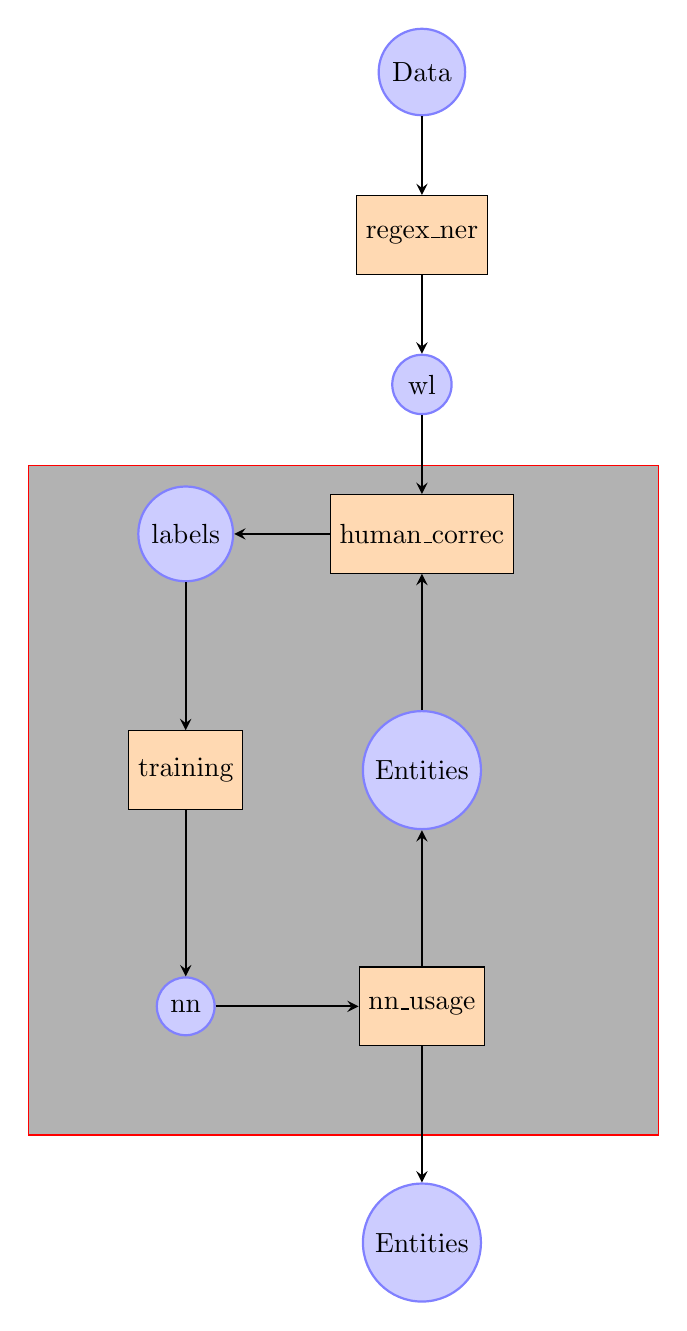
\begin{tikzpicture}[node distance=3cm]
		%\begin{tikzpicture}%[->,shorten >=1pt,auto,node distance=2.8cm,semithick]
			\node (data) [state] {Data};
			\node (module0) [process, below=1cm of data] {regex\_ner};
			\draw [arrow] (data) -- (module0);
			\node (wl) 		[state, below=1cm of module0] {wl};
			\draw [arrow] (module0) -- (wl);
			\node (humcorr) [process, below=1cm of wl] {human\_correc};
			\draw [arrow] (wl) -- (humcorr);
			\node (l) 		[state, left of=humcorr] {labels};
			\draw [arrow] (humcorr) -- (l);
			\node (train) 	[process, below of=l] {training};
			\draw [arrow] (l) -- (train);
			\node (nn) 		[state, below of=train] {nn};
			\draw [arrow] (train) -- (nn);
			\node (module) [process, right of=nn] {nn\_usage};
			\draw [arrow] (nn) -- (module);
			\node (entities) [state, below of=module] {Entities};
			\node (entitiescorr) [state, above of=module] {Entities};
			\draw [arrow] (module) -- (entities);
			\draw [arrow] (module) -- (entitiescorr);
			\draw [arrow] (entitiescorr) -- (humcorr);
			
\begin{pgfonlayer}{background}
\filldraw [fill=black!30,draw=red] (3,-5) rectangle (-5,-13.5);
%\filldraw [fill=black!30,draw=red] (nn.south -| nn.west) rectangle (humcorr.north -| entitiescorr.east);
\end{pgfonlayer}
		\end{tikzpicture}
		\caption{Human In The Loop framework} % caption
		%\label{fig:diagram}             % for referencing of figure, key select as you wish
	\end{figure}
\end{comment}



Configuriamo l'uso delle componenti regex, \acrshort{machine-learning}, task di creazione regex e task di 
annotazione manuale come un sistema di tipo \acrshort{human-in-the-loop}.
In tale sistema l'essere umano pu� essere utilizzato come programmatore di regex e come annotatore a pi� riprese successive.
Partendo dallo studio \say{How to invest my time} \cite{HowToInvestMyTime}, l'indicazione che traiamo per usare al meglio
il lavoro umano � investire pochi minuti sulla creazione di regex ad alta \acrlong{Recall} per poi effettuare la correzione umana delle annotazioni prodotte dalla regex stessa.
Seguendo la convenzione dello studio citato, chiameremo \say{weak labelling} l'estrazione svolta con la regex, che indicheremo con \(RE\sb{WL}\): le label cos� prodotte risultano \say{weak}, ossia non verificate e passibili d'errore.
%La \textbf{human annotation} prender� in input le \textbf{weak labels} prodotte con la  \(RE\sb{WL}\)
%e produrr� annotazioni che potremo considerare affidabili perch� verificate da un umano;
%tali annotazioni costituiranno il training set della rete neurale.
L'attivit� umana \textbf{\(correct\sb{k}labels\)}, partendo dalle weak labels come input iniziale \(labels\sb{0}\), ad ogni iterazione \textit{i} apporter� \textit{k} correzioni che andranno a formare l'insieme di labels \(labels\sb{i}\). Qualora il ciclo continui, tale insieme i-esimo potr� essere adoperato come input dell'iterazione \textit{i+1}; in caso contrario verr� assunto come training set per istruire la rete neurale.


%\begin{left}
\includegraphics[ clip, width=\textwidth,height=\textheight,keepaspectratio]{PlotFunctionData_30+.pdf} 
\caption{Human In The Loop: F1-score, Precision e Recall.} 
\label{fig:hitl}
%\end{left}

L'uso dello \acrlong{human-in-the-loop} pu� essere vantaggioso se effettuato in maniera tale da:
\begin{itemize}
\item istruire una rete neurale in un tempo minimo di lavoro umano;  
\item permettere il fine-tuning della rete neurale stessa
con l'intervento dell'annotatore umano.
\end{itemize}

Seguendo dunque lo studio gi� citato, l'operatore umano deve destinare pochi minuti alla realizzazione delle  regex \(RE\sb{WL}\). Nella nostra prova utilizziamo le regex \[regex-soa\sb{wl-v1}=\textsc{\char13}O(S|G)(\\d\\d?)\textsc{\char13} \]  \[ regex-class\sb{wl-v1}=\textsc{\char13}(IV|IV|III|II|IX|VIII|VII|VI|X|V|I)\textsc{\char13} \] realizzate in pochi minuti su un tool di regex-editing liberamente disponibile online. Usando tali regex abbiamo quindi prodotto le weak labels che vanno a formare il dataset iniziale \(labels\sb{0}\);
per ogni iterazione successiva \(i>0\) vengono 
 dunque corrette \textit{k} annotazioni weak con \(k=100\). Il grafico \ref{fig:hitl} illustra l'evoluzione del sistema \acrshort{human-in-the-loop} all'aumentare 
delle correzioni umane apportate alle weak labels: viene
rappresentato il guadagno in termini di \acrlong{Precision}, \acrlong{Recall} e \acrlong{F1-score}.
In vari esperimenti analoghi a quello riportato in figura \ref{fig:hitl} si evince come in dieci iterazioni di correzione il %sistema guadagni oltre il 22\% di \acrlong{Precision}, 34\% di \acrlong{Recall} e 32\% di \acrlong{F1-score}.
sistema valutato in termini di  \acrshort{Precision}, \acrshort{Recall}, \acrshort{F1-score} riporti i guadagni minimi:
\[\Delta\sb{i=10}(P,R,F1)=(22\%,34\%, 32\%)\]
� interessante notare come alla settima iterazione correttiva tali guadagni ammontano gi� al
\[\Delta\sb{i=7}(P,R,F1)=(21\%,33\%, 31\%)\]
Portando il discorso ai risultati specifici dell'esperimento al grafico \ref{fig:hitl}, l'iterazione numero dieci porta ai valori \[[P,R,F]\sb{NER-HITL}=[0.8458, 0.7071, 0.7527 ] \] a fronte dei valori 
del sistema NER-ML costruito sulla \textit{ground truth} \[[P,R,F]\sb{NER-ML}= [0.8476, 0.7778, 0.7973] \]. In figura 
\ref{fig:ist} possiamo vedere graficamente il confronto tra \textit{NER-HITL} e \textit{NER-ML}.%\includegraphics[ clip, width=\textwidth,height=\textheight,keepaspectratio]{PlotFunctionData_hitl_vs_ml.pdf} \caption{} \label{fig:hitlvsml}



\center
\includegraphics[width=0.9\linewidth, height=6cm]{PlotFunctionData_hitl_vs_ml.pdf}
\caption{Grafico comparativo di NER-HITL-v1 e NER-ML}
\label{fig:ist}
\center
% ML 0.847669252797008	0.777828714411617	0.797399765346802
% p 21 r 33 f 31 segna come iterazione 7
% p 25 r 34 f 32 (_v1_29_n)
% p 22 r 38 f 35 (_v1_30_n+)
% p 25 r 36 f 34 (_v1_30_n)
% hitl p 0.845849682049472 r 0.707145200862464 f 0.752779411712778
% gold p 0.847669252797008 r 0.777828714411617 f 0.797399765346802

% !TEX encoding = IsoLatin 

% Affinch� gli accenti vengano accettati, assicurati che la codifica di questo file
% sia ISO 8859-1

% PER OTTENERE IL PDF, digitare da terminale
% ./makepdfplease
% 

\chapter{Conclusioni}
Scopo di questa tesi � stato effettuare un task di Named Entity Recognition 
su documenti provenienti dalla pubblica amministrazione; tale set di documenti,
rumorosi in un quanto spesso ottenuti via OCR a partire da documenti stampati,
risulta spesso descrivere gli stessi dati formali con diciture variabili.
� stata presentata l'implementazione del task di NER con l'uso di regex,
ma � apparso chiaro come questo approccio risulti difficile da migliorare nel tempo;
infatti le regex alla modifica risultano error-prone e di difficile manutenzione e documentazione,
caratteristiche che non aiutano ad esprimere pattern molto variabili.
D'altro canto � stato presentato un NER che adopera tecniche di supervised deep learning
e che meglio si adegua ad estrarre dati variabili, a spese tuttavia di un
ingente tempo umano di annotazione.
� apparsa dunque conveniente la possibilit� di effettuare una \say{weak supervision}
adoperando un dataset prodotto dal task di NER-regex;
tale dataset viene prodotto in pochi minuti, dopodich� � sottoposto a cicliche iterazioni di correzione
da parte di un annotatore umano. Il loop di addestramento cos� configurato � detto Human In The Loop.
Abbiamo notato come l'operatore umano sia significativamente pi� veloce nel compito di 
\textit{correzione-annotazione} rispetto al compito di produzione di annotazioni \textit{from scratch}.
Valutando le perfomance di NER-hitl-i al variare dell'iterazione i-esima, � emerso che:
� possibile ottenere un risultato subottimale con la sola \textit{annotazione-correzione} di 1000 annotazioni,
sacrificando 7\% di recall ma comunque risparmiando pi� del 70\% del tempo d'annotazione.
Infine, portando le iterazioni di NER-hitl-i a 14 � possibile superare le prestazioni di NER-ML,
adoperando comunque il 10\% di annotazioni in meno e risparmiando un tempo di annotazione pari a 58\%.
� possibile immaginare dei futuri miglioramenti per lo schema Human In The Loop individuato;
in particolare si potrebbe fornire all'annotatore una metrica per calcolare quali porzioni di testo
sono pi� rumorose e probabilmente pi� prioritarie rispetto al task di annotazione-correzione .

\backmatter
\printglossary[type=\acronymtype]

% bibliografia scritta "a mano"
%\input{biblio.tex}
% se la bibliografia � stata scritta (usando Bibtex) nel file biblio.bib allora commentare la riga precedente e scommentare le due righe seguent
\bibliographystyle{plain} 
\bibliography{biblio.bib}

\end{document}
